\chapter{Linear models}
\label{chap:linear_models}

\begin{supportbox}{About this chapter}
Programming software is done by choosing the appropriate sequence of primitive operations to solve a task. By analogy, building a model is done by choosing the correct sequence of \textit{differentiable} blocks. In this chapter we introduce the simplest possible block, so-called linear models, which assume that inputs act additively on the output via a weighted average. In a sense, all differentiable models are smart variations and compositions of linear blocks.
\end{supportbox}

\section{Least-squares regression}

\subsection{Problem setup}

Summarizing the previous chapter, a supervised learning problem can be defined by choosing the input type $x$, the output type $y$, the model $f$, and the loss function $l$. In this chapter we consider the simplest possible choices for all of them, namely:
%
\begin{itemize}
    \item The input is a vector $\mathbf{x} \sim (c)$, corresponding to a set of features (e.g., $c$ personal features of a client of a bank). We use the scalar $c$ (short for \textit{channels}) to denote the number of features to be consistent with the following chapters.
    \item The output is a single real value $y \in \mathbb{R}$. In the unconstrained case, we say this is a \textbf{regression} task. If $y$ can only take one out of $m$ possible values, i.e., $y \in \left\{1, \ldots, m\right\}$, we say this is a \textbf{classification} task. In the special case of $m=2$, we say this is a \textbf{binary classification}  task.
    \item We take $f$ to be a linear model, providing us with simple closed-form solutions in some cases, most notably \textbf{least-squares regression} (Section \ref{subsec:least_squares}).
\end{itemize}
%
The basic shapes to remember are summarized in Table \ref{tab:shapes}. We begin by discussing the choice of loss in the regression case. We start from the regression case since, as we show later, classification can be solved by small modifications to the regression case.

\begin{table}[t]
\centering
\caption{Basic shapes to remember for this chapter. For uniformity, we will use the same letters as much as possible throughout the book.}
\begin{tabular}{@{}cl@{}}
\toprule
 $n$ & \textbf{size of the dataset} \\ $c$ & \textbf{features} \\ $m$ & \textbf{classes}\\ \midrule
\end{tabular}
\label{tab:shapes}
\end{table}

\subsection{Regression losses: the squared loss and variants}

Finding a loss for regression is relatively simple, since the prediction error $e = (\hat{y} - y)$ between the predicted output of the model $\hat{y} = f(x)$ and the true desired output $y$ is a well-defined target, being a continuous function of the model’s output that decreases monotonically. Since in general we do not care about the sign of the prediction error, a common choice is the \textbf{squared loss}:

\begin{equation}
    l(\hat{y},y)=(\hat{y}-y)^2
    \label{eq:squared_loss}
\end{equation}

Here and in the following we use the symbol $\hat{y}$ to denote the prediction of a generic model. As we will see, working with \eqref{eq:squared_loss} provides a number of interesting benefits to our solution. Among others, the gradient of the squared loss is a linear function of the model’s output, allowing us to solve it in closed-form for the optimal solution. 

Recalling the maximum likelihood principle (Section \ref{sec:maximum_likelihood_estimation}), the squared loss can be obtained by assuming that the outputs of the model follow a Gaussian distribution centered in $f(\mathbf{x})$ and with a constant variance $\sigma^2$:

$$
p(y \;\vert\; f(\mathbf{x}))=\mathcal{N}(y\;\vert\;f(\mathbf{x}), \sigma^2)
$$

In this case the log-likelihood (for a single point) can be written as:\footnote{Recalling that $\log(ab)=\log(a)+\log(b)$ and $\log(a^b)=b\log(a)$.}

\begin{equation}
\log(p(y \mid f(\mathbf{x}), \sigma^2)) = -\log(\sigma) - \frac{1}{2}\log(2\pi) - \frac{1}{2\sigma^2}(y - f(\mathbf{x}))^2
\label{eq:ls_maximum_likelihood}
\end{equation}

Minimizing \eqref{eq:ls_maximum_likelihood} for $f$, we see that the first two terms on the right-hand side are constant, and the third reverts to the squared loss. Minimizing for $\sigma^2$ can be done independently from the optimization of $f$, with a simple closed-form solution (see below, equation \eqref{eq:ls_sigma}).

Coming up with variants to the squared loss is also easy. For example, one drawback of the squared loss is that higher errors will be penalized with a strength that grows quadratically in the error, which may provide undue influence to \textbf{outliers}, i.e., points that are badly mislabeled. Other choices that diminish the influence of outliers can be the \textbf{absolute value loss} $l(\hat{y}, y) = \lvert \hat{y} - y \rvert$ or the Huber loss (a combination of the squared loss and the absolute loss):
%
\begin{equation}
\text{Huber loss: } L(y, \hat{y}) = \begin{cases} \frac{1}{2}\left(y - \hat{y}\right)^2 & \text{ if } \lvert y - \hat{y} \rvert \le 1 \\ \left(\lvert y - \hat{y} \rvert - \frac{1}{2}\right) & \text{ otherwise } \end{cases}
\end{equation}
%
\begin{SCfigure}
    \centering
    \hspace{1em}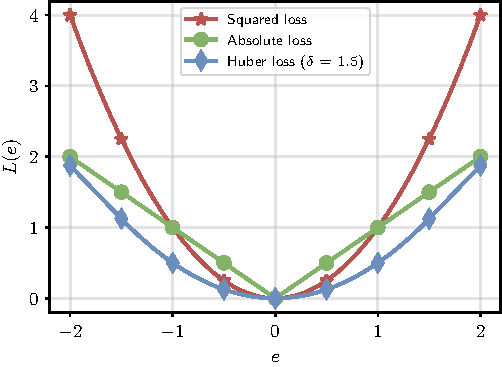
\includegraphics[width=0.6\textwidth]{images/loss_functions_regression.pdf}
    \caption{Visualization of the squared loss, the absolute loss, and the Huber loss with respect to the prediction error $e = (\hat{y} - y)$.}
    \label{fig:losses_regression}
\end{SCfigure}

which is quadratic in the promixity of $0$ error, and linear otherwise (with the $-\frac{1}{2}$ term added to ensure continuity). See Figure \ref{fig:losses_regression} for a visualization of these losses with respect to the prediction error. 

The absolute loss seems an invalid choice in our context, since it has a point of non-differentiability in $0$ due to the absolute value. We will see later that functions with one (or a small number) of points of this form are not truly problematic. Mathematically, they can be handled by the notion of \textbf{subgradient} (a slight generalization of the derivative). Practically, you can imagine that if we start from a random initialization, gradient descent will never reach these points with perfect precision, and the derivatives of $\lvert \varepsilon \rvert$ for any $\varepsilon > 0$ is always defined.

\subsection{The least-squares model}
\label{subsec:least_squares}

\addclock With a loss function in hand, we consider the following model (a linear model) to complete the specification of our first supervised learning problem.
%
\begin{definition}[Linear models] 
A \textbf{linear model} on an input $\mathbf{x}$ is defined as:
%
$$
f(\mathbf{x})=\mathbf{w}^\top\mathbf{x} + b
$$
%
where $\mathbf{w} \sim (c)$ and $b \in \mathbb{R}$ (the \textit{bias}) are trainable parameters.
\end{definition}

The intuition is that the model assigns a fixed weight $w_i$ to each input feature $x_i$, and provides a prediction by linearly summing all the effects for a given input $\mathbf{x}$, reverting to a default prediction equal to $b$ whenever $\mathbf{x} = \mathbf{0}$. Geometrically, the model defines a line for $d=1$, a plane for $d=2$, and a generic hyperplane for $d > 1$. From a notational perspective, we can sometimes avoid writing  a bias term by assuming a constant term of $1$ as the last feature of $\mathbf{x}$:
%
$$
f\left(\begin{bmatrix}\mathbf{x}\\1\end{bmatrix}\right) = \mathbf{w}^\top\begin{bmatrix}\mathbf{x}\\1\end{bmatrix} = \mathbf{w}_{1:c}^\top\mathbf{x}+w_{c+1}
$$

Combining the linear model, the squared loss, and an empirical risk minimization problem we obtain the \textbf{least-squares optimization problem}.

\begin{definition}[Least-squares] \addbottle
The \textbf{least-squares} optimization problem is given by:
%
\begin{equation}
\mathbf{w}^*, b^* = \underset{\mathbf{w}, b}{\arg\min} \;\;\frac{1}{n}\sum_{i=1}^n \left(y_i - \mathbf{w}^\top \mathbf{x}_i - b\right)^2
\label{eq:least_squares}
\end{equation}
\end{definition}

Before proceeding to the analysis of this problem, we rewrite the least-squares in a \textbf{vectorized} form that only involves matrix operations (matrix products and norms). This is useful because, as already stated, modern code for training differentiable models is built around $n$-dimensional arrays, with optimized hardware to perform matrix operations on them. To this end, we first stack all the inputs and outputs of our training set into an \textbf{input matrix}:

$$
\mathbf{X} = \begin{bmatrix} \mathbf{x}_1^\top \\ \vdots \\ \mathbf{x}_n^\top \end{bmatrix} \sim (n,c)
$$

and a similar \textbf{output vector} $y = \left[ y_1, \ldots, y_n\right]^\top$. We can write a batched model output (the model output for a mini-batch of values) as:

\begin{equation}
f(\mathbf{X})=\mathbf{X}\mathbf{w} + \eqnmarkbox[drawblue]{node}{\mathbf{1}b}
\label{eq:batched_linear_model}
\end{equation}
\annotate[yshift=-1em]{below,right}{node}{Same bias $b$ for all $n$ predictions}

\vspace{1em}
Equations like \eqref{eq:batched_linear_model} can be replicated almost line-by-line in code - see Box \ref{code:linear_model} for an example in PyTorch. 

\begin{mypy}{Computing a batched linear model as in \protect\eqref{eq:batched_linear_model}. For clarity, we are showing the array dimensions as type hints using {\footnotesize \texttt{jaxtyping} (\url{https://docs.kidger.site/jaxtyping/})}.}{code:linear_model}
def linear_model(w: Float[Tensor, "c"],
                 b: Float,
                 X: Float[Tensor, "n c"]) 
                 -> Float[Tensor, "n"]:
  return X @ w + b
\end{mypy}

Of only marginal interest for now but of more importance for later, we note that the row ordering of the input matrix and of the output vector are fundamentally arbitrary, in the sense that permuting their rows will only result in a corresponding permutation of the rows of $f(\mathbf{X})$. This is a simple example of a phenomenon called \textbf{permutation equivariance} that will play a much more important role later on.

The vectorized least-squares optimization problem becomes:
%
\begin{equation}
\text{LS}(\mathbf{w},b) =  \frac{1}{n} \left\lVert \mathbf{y} - \mathbf{X}\mathbf{w} - \mathbf{1}b \right\rVert^2 
\label{eq:ls_vectorized}
\end{equation}
%
where we recall that the norm of a vector is defined as $\lVert \mathbf{e} \rVert^2 = \sum_i e_i^2$.

\subsection{Solving the least-squares problem}

To solve the least-squares problem through gradient descent, we need the equations for its gradient. Although we will soon develop a general algorithmic framework to compute these gradients automatically (Chapter \ref{chap:automatic_differentiation}), it is instructive to look at the gradient itself in this simple scenario. Ignoring the bias (for the reasons stated above, we can incorporate it in the weight vector), and other constant terms we have:
%
$$
\nabla \text{LS}(\mathbf{w}) = \mathbf{X}^\top\left( \mathbf{X}\mathbf{w} - \mathbf{y} \right)
$$
%
The LS problem is convex in the weights of the model, as can be understood informally by noting that the equations describe a paraboloid in the space of the weights (a quadratic function). The global minima are then described by the equations:
%
$$
\mathbf{X}^\top\left( \mathbf{X}\mathbf{w} - \mathbf{y} \right) = 0 \;\;\Rightarrow\;\; \mathbf{X}^\top\mathbf{X}\mathbf{w} = \mathbf{X}^\top\mathbf{y}
$$

\begin{mypy}{Solving the least-squares problem with the closed-form solution. The numerically stable variant calls a solver specialized for systems of linear equations.}{code:ls_closed_form}
def least_squares_solve(w: Float[Tensor, "c"],
                        X: Float[Tensor, "n c"],
                        y: Float[Tensor, "n"],
                        numerically_stable = True) \
                        -> Float[Tensor, "c"]:
  # Explicit solution
  if not numerically_stable:
    return torch.linalg.inv(X.T @ X) @ X.T @ y 
  else:
    return torch.linalg.solve(X.T @ X, X.T @ y)
\end{mypy}

These are called the \textbf{normal equations}. Importantly, the normal equations describe a linear system of equations in $\mathbf{w}$,\footnote{That is, we can write them as $\mathbf{A}\mathbf{w}=\mathbf{b}$, with $\mathbf{A} = \mathbf{X}^\top\mathbf{X}$ and $\mathbf{b} = \mathbf{X}^\top\mathbf{y}$.} meaning that under the appropriate conditions (invertibility of $\mathbf{X}^\top\mathbf{X}$) we can solve for the optimal solution as:
%
\begin{equation}
\mathbf{w}_*=\left(\mathbf{X}^\top\mathbf{X}\right)^{-1}\mathbf{X}^\top\mathbf{y}
\label{eq:ls_closed_form_solution}
\end{equation}

\begin{supportbox}{Tidbits of information}
The matrix $\mathbf{X}^\dagger=\left(\mathbf{X}^\top\mathbf{X}\right)^{-1}\mathbf{X}^\top$ is called the \textbf{pseudoinverse} (or \textbf{Moore-Penrose inverse}) of the non-square matrix $\mathbf{X}$, since $\mathbf{X}^\dagger\mathbf{X}=\mathbf{I}$. Performing the inversion in \eqref{eq:ls_closed_form_solution} is not always possible: for example, if one feature is a scalar multiple of the other, the matrix $\mathbf{X}$ does not have full rank (this is called \textbf{collinearity}). Finally, note that the predictions of the least-squares model can be written as $\hat{\mathbf{y}}=\mathbf{M}\mathbf{y}$, with $\mathbf{M} = \mathbf{X}\mathbf{X}^\dagger$. Hence, least-squares can also be interpreted as performing a weighted average of the training labels, where the weights are given by a projection on the column space induced by $\mathbf{X}$. This is called the \textbf{dual} formulation of least-squares. Dual formulations provide an intrinsic level of debugging of the model, as they allow to check which inputs were the most relevant for a prediction by checking the corresponding dual weights \cite{irie2022dual}. 
\end{supportbox}

This is the only case in which we will be able to express the optimal solution in a closed-form way, and it is instructive to compare this solution with the gradient descent one. To this end, we show in Box \ref{code:ls_closed_form} an example of solving the least-squares in closed form using \eqref{eq:ls_closed_form_solution}, and in Box \ref{code:ls_gradient_descent} the equivalent gradient descent formulation. A prototypical evolution of the loss in the latter case is plotted in Figure \ref{fig:loss_evolution}. Since we selected a very small learning rate, each step in the gradient descent procedure provides a stable decrease in the loss, until convergence. Practically, convergence could be checked by numerical means, e.g., by evaluating the difference in norm between two iterations for some numerical threshold $\varepsilon > 0$:
%
\begin{equation}
    \lVert \mathbf{w}_{t+1} - \mathbf{w}_t \rVert^2 < \varepsilon
\end{equation}
%
As we will see, understanding when more complex models have converged will be a more subtle task.

Considering again the Gaussian log-likelihood in \eqref{eq:ls_maximum_likelihood}, we can also optimize the term with respect to $\sigma^2$ once the weights have been trained, obtaining:
%
\begin{equation}
\sigma_*^{2} = \frac{1}{n}\sum_{i=1}^n (y_i - \mathbf{w}_*^{\top}\mathbf{x}_i)^2 \,.
\label{eq:ls_sigma}
\end{equation}
%
which has the intuitive meaning that the variance of the model is constant (by definition) and given by the average squared prediction error on our training data. More sophisticated probabilistic models can be obtained by assuming the variance itself is predicted by the model (\textbf{heteroscedastic} models), see \cite{bishop2006pattern}.

\begin{mypy}{Same task as Box \protect\ref{code:ls_closed_form}, solved with a naive implementation of gradient descent with a fixed learning rate that defaults to $\eta = 0.001$.}{code:ls_gradient_descent}
def least_squares_gd(X: Float[Tensor, "n c"],
                     y: Float[Tensor, "n"],
                     learning_rate=1e-3) \
                     -> Float[Tensor, "c"]:
    # Initializing the parameters
    w = torch.randn((X.shape[1], 1))

    # Fixed number of iterations
    for i in range(15000):
      # Note the sign: the derivative has a minus!
      w = w + learning_rate * X.T @ (y - X @ w)

    return w
\end{mypy}

\begin{SCfigure}
    \centering
    \hspace{1em} 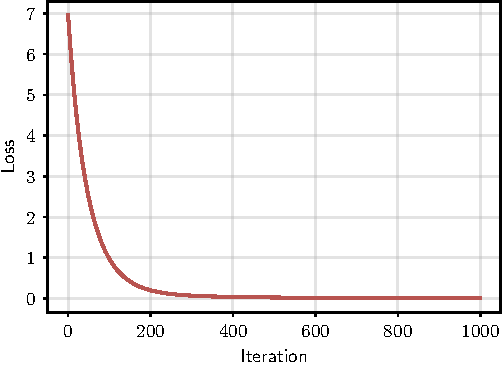
\includegraphics[width=0.5\textwidth]{images/least_squares_example.pdf}
    \caption{An example of running code from Box \ref{code:ls_closed_form}, where the data is composed of $n=10$ points drawn from a linear model $\mathbf{w}^\top \mathbf{x} + \varepsilon$, with $w_i \sim \mathcal{N}(0, 1)$ and $\varepsilon \sim \mathcal{N}(0, 0.01)$. Details apart, note the very smooth descent: each step provides a decrease in loss.}
    \label{fig:loss_evolution}
\end{SCfigure}


\subsection{Some computational considerations}

\addteacup Even if the inverse can be computed, the quality of the solution will depend on the condition number of $\mathbf{X}^\top\mathbf{X}$, and large numerical errors can occur for poorly conditioned matrices.\footnote{The condition number of a matrix $\mathbf{A}$ is defined as $\kappa(\mathbf{A}) = \lVert\mathbf{A}\rVert\lVert\mathbf{A}^{-1}\rVert$ for some choice of matrix norm $\lVert \bullet \rVert$. Large conditions number can make the inversion difficult, especially if the floating-point precision is not high.} In addition, the computational cost of solving \eqref{eq:ls_closed_form_solution} may be prohibitive. The matrix inversion will scale, roughly, as $\mathcal{O}(c^3)$. As for the matrix multiplications, the algorithm requires a multiplication of a $c \times n$ matrix with another $n \times c$ one, and a multiplication between a $c \times c$ matrix and a $c \times n$ one. Both these operations will scale as $\mathcal{O}(c^2n)$.

In general, we will always prefer algorithms that scale linearly both in the feature dimension $c$ and in the batch size $n$, since super-linear algorithms will become quickly impractical (e.g., a batch of $32$ RGB images of size $1024 \times 1024$ has $c \approx 1e^{7}$). We can avoid a quadratic complexity in the equation of the gradient by computing the multiplications in the correct order, i.e., computing the matrix-vector product $\mathbf{X}\mathbf{w}$ first. Hence, pure gradient descent is linear in both $c$ and $n$, but only if proper care is taken in the implementation: generalizing this idea is the fundamental insight for the development of \textbf{reverse-mode automatic differentiation}, a.k.a. \textbf{back-propagation} (Section \ref{sec:reverse_mode_automatic_differentiation}).

\subsection{Regularizing the least-squares solution}
\label{subsec:regularizing_least_squares}

Looking again at the potential instability of the inversion operation, suppose we have a dataset for which the matrix is almost singular, but we still wish to proceed with the closed-form solution. In that case, it is possible to slightly modify the problem to achieve a solution which is “as close as possible” to the original one, while being feasible to compute. For example, a known trick is to add a small multiple, $\lambda > 0$, of the identity matrix to the matrix being inverted:
%
$$
\mathbf{w}^*=\left(\mathbf{X}^\top\mathbf{X} {\color{drawred}+\lambda\mathbf{I}}\right)^{-1}\mathbf{X}^\top\mathbf{y}
$$
%
This pushes the matrix to be “more diagonal” and improves its condition number. Backtracking to the original problem, we note this is the closed form solution of a modified optimization problem:
%
$$
\text{LS-Reg}(\mathbf{w}) =  \frac{2}{n} \left\lVert \mathbf{y} - \mathbf{X}\mathbf{w} \right\rVert^2 {\color{drawred}+ \frac{\lambda}{2}\lVert \mathbf{w} \rVert^2}
$$
%
This problem is called \textbf{regularized least-squares} (or \textbf{ridge regression}), and the red part in the loss is an instance of $\ell_2$-regularization (or, more generally, regularization). Note that regularization does not depend on the dataset, as it simply encodes a preference for a certain type of solution (in this case, low-norm weights), where the strength of the preference itself is defined by the hyper-parameter $\lambda$. From a Bayesian perspective (Section \ref{sec:bayesian_learning}), the regularized least-squares corresponds to a MAP solution when defining a Gaussian prior over the weights centered in zero with constant variance.

\section{Linear models for classification}
\label{sec:linear_models_for_classification}

We now move to classification, in which $y_i \in \left\{1, \ldots, m\right\}$, where $m$ defines the number of \textbf{classes}. As we will see later, this is a widely influential problem, encompassing a range of tasks in both computer vision (e.g., image classification) and natural language processing (e.g., next-token prediction). We can tackle this problem by slight variations with respect to the regression case.

While we can solve the task by regressing directly on the integer value $y_i$, it is instructive to consider why this might not be a good idea. First, it is difficult for a model to directly predict an integer value, since this requires some thresholding that would render its gradient zero almost everywhere. Instead, we could regress on a real value $\widetilde{y}_i \in \left[1, m\right]$ inside the interval from $1$ to $m$ (as we will show, bounding the output of the model inside an interval can be done easily). During inference, given the output $\hat{y}_i = f(\mathbf{x}_i)$, we map back to the original domain by rounding:
%
$$
\text{Predicted class} =\text{round}(\hat{y}_i)
$$
%
For example, $\hat{y}_i = 1.3$ would be mapped to class $1$, while $\hat{y}_i = 3.7$ would be mapped to class $4$. Note that this is a post-hoc processing of the values that is only feasible at inference time. The reason this is not a good modelling choice is that we are introducing a spurious ordering of the classes which might be exploited by the model itself, where class $2$ is “closer” to class $3$ than it is to class $4$. We can avoid this by moving to a classical \textbf{one-hot encoded} version of $y$, which we denote by $\mathbf{y}^{\text{oh}} \sim \text{Binary}(m)$:
%
$$
\idx{\mathbf{y}^{\text{oh}}}{j}=\begin{cases} 1 &\text{ if } y = j \\ 0 & \text{ otherwise} \end{cases}
$$
%
For example, in the case of three classes, we would have $\mathbf{y}^{\text{oh}} = \left[1 \;\; 0 \;\; 0 \right]^\top$ for class $1$, $\mathbf{y}^{\text{oh}} = \left[0 \;\; 1 \;\; 0 \right]^\top$ for class $2$, and $\mathbf{y}^{\text{oh}} = \left[0 \;\; 0 \;\; 1 \right]^\top$ for class $3$ (this representation should be familiar to readers with some background in machine learning, as it is a standard representation for categorical variables). 

One-hot vectors are unordered, in the sense that given two generic outputs $\mathbf{y}_1^{\text{oh}}$ and $\mathbf{y}_2^{\text{oh}}$, their Euclidean distance is either $0$ (same class) or $\sqrt{2}$ (different classes). While we can perform a multi-valued regression directly on the one-hot encoded outputs, with the mean-squared error known as the \textbf{Brier score} in this case, we show below that a better and more elegant solution exists, in the form of \textbf{logistic regression}.

\subsection{The probability simplex and the softmax function}
\label{sec:softmax}

We cannot train a model to directly predict a one-hot encoded vector (for the same reasons described above), but we can achieve something similar by a slight relaxation. To this end, we re-introduce the \textbf{probability simplex}.

\begin{definition}[Probability simplex]
The \textbf{probability simplex} $\Delta_n$ is the set of vectors $\mathbf{x} \sim \Delta(n)$ such that:
%
$$
x_i \ge 0, \; \sum_i x_i=1
$$
%
\end{definition}

Geometrically, you can picture the set of one-hot vectors as the vertices of an $n$-dimensional polytope, and the simplex as its convex hull: values inside the simplex, such as $[0.2, 0.05, 0.75]$, do not precisely correspond to a vertex, but they allow for gradient descent because we can smoothly move inside the polytope. Given a value $\mathbf{x} \in \Delta_n$, we can project to its closest vertex (the predicted class) as:
%
$$
\underset{i}{\arg\max} \left\{ \mathbf{x}_i \right\}
$$
%
As the name implies, we can interpret values inside the simplex as probability distributions, and projection on the closest vertex as finding the mode (the most probable class) in the distribution. In this interpretation, a one-hot encoded vector is a “special case” where all the probability mass is concentrated on a single class (which we know to be the correct one).

In order to predict a value in this simplex, we need two modifications to the linear model from \eqref{eq:least_squares}: first, we need to predict an entire vector simultaneously; and second, we need to constrain the outputs to lie in the simplex. First, we modify the linear model to predict an $m$-dimensional vector:
%
\begin{equation}
\mathbf{y} =\mathbf{W}\mathbf{x}+\mathbf{b}
\label{eq:multi_valued_linear_model}
\end{equation}
%
where $\mathbf{W} \sim (m,c)$ can be interpreted as $m$ linear regression models running in parallel, and $\mathbf{b} \sim(m)$. This output is unconstrained and it is not guaranteed to be in the simplex. The idea of logistic regression is to combine the linear model in \eqref{eq:multi_valued_linear_model} with a simple, parameter-free transformation that projects inside the simplex, called the \textbf{softmax} function.

\begin{definition}[Softmax function] \addbottle
The \textbf{softmax} function is defined for a generic vector $\mathbf{x} \sim(m)$ as:

\begin{equation}
\idx{\textnormal{softmax}(\mathbf{x})}{i} = \frac{\exp(x_i)}{\sum_j\exp(x_j)}
\label{eq:softmax}
\end{equation}

\end{definition}

Let us decompose the terms in \eqref{eq:softmax} into the basic computations that are executed by introducing two intermediate terms. First, the numerator of the softmax converts each number to a positive value $h_i$ by exponentiation:
%
\begin{equation}
h_i =\exp(x_i)
\end{equation}
%
Second, we compute a normalization factor $Z$ as the sum of these new (non-negative) values:
%
\begin{equation}
 Z = \sum_jh_j 
 \end{equation}
%
The output of the softmax is then given by dividing $h_i$ by $Z$, thus ensuring that the new values sum to $1$:
%
\begin{equation}
y_i = \frac{h_i}{Z}
\end{equation}

Another perspective comes from considering a more general version of the softmax, where we add an additional hyper-parameter $\tau > 0$ called the \textbf{temperature}:

$$
\text{softmax}(\mathbf{x};\tau)=\text{softmax}(\mathbf{x}/\tau)
$$

The softmax keeps the relative ordering among the values of $x_i$ for all values of $\tau$, but their absolute distance is increased or decreased based on the temperature. In particular, we have the following two limiting cases:

\begin{gather}
\lim_{\tau \rightarrow \infty} \text{softmax}(\mathbf{x};\tau)=1/c \\ 
\lim_{\tau \rightarrow 0} \text{softmax}(\mathbf{x};\tau)=\underset{i}{\arg\max} \;\; \mathbf{x}
\end{gather}

For infinite temperature, relative distances will disappear and the output reverts to a uniform distribution. At the contrary, at $0$ temperature the softmax reverts to the (poorly differentiable) argmax operation. Hence, softmax can be seen as a simple differentiable approximation to the argmax, and a better name should be \textbf{softargmax}. However, we will retain the most standard name here. See Figure \ref{fig:softmax} for a visualization of a softmax applied on a generic three-dimensional vector with different temperature values.

\begin{figure}[t]
    \centering
    \begin{subfigure}[b]{0.24\textwidth}
    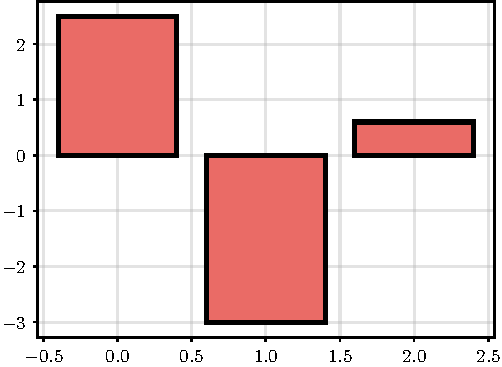
\includegraphics[width=\textwidth]{images/softmax_1.pdf}
    \caption{Inputs}
    \end{subfigure}
    \hfill
    \begin{subfigure}[b]{0.24\textwidth}
    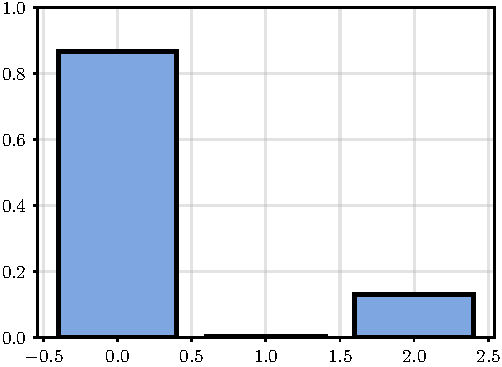
\includegraphics[width=1.0\textwidth]{images/softmax_2.pdf}
    \caption{$\tau=1$}
    \end{subfigure}
    \hfill
    \begin{subfigure}[b]{0.24\textwidth}
    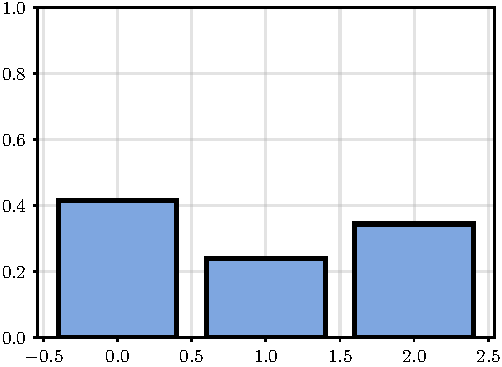
\includegraphics[width=1.0\textwidth]{images/softmax_3.pdf}
    \caption{$\tau=10$}
    \end{subfigure}
    \hfill
    \begin{subfigure}[b]{0.24\textwidth}
    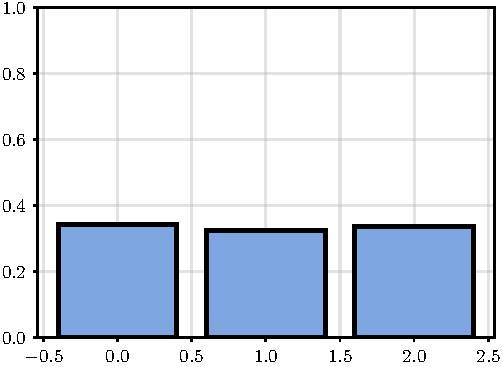
\includegraphics[width=1.0\textwidth]{images/softmax_4.pdf}
    \caption{$\tau=100$}
    \end{subfigure}
    \hfill
    \caption{Example of softmax applied to a three-dimensional vector (a), with temperature set to 1 (b), 10 (c), and 100 (d). As the temperature increases, the output converges to a uniform distribution. Note that inputs can be both positive or negative, but the outputs of the softmax are always constrained in $[0,1]$.}
    \label{fig:softmax}
\end{figure}


\subsection{The logistic regression model}
\label{subsec:logistic_regression}

\addclock We can summarize our previous discussion by combining the softmax in \eqref{eq:softmax} with the linear model in \eqref{eq:multi_valued_linear_model} to obtain a linear model for classification:

$$
\hat{\mathbf{y}}=\text{softmax}\left(\mathbf{W}\mathbf{x} + \mathbf{b}\right)
$$

The pre-normalized outputs $\mathbf{h} = \mathbf{W}\mathbf{x}+\mathbf{b}$ are called the \textbf{logits} of the model, a name that will be discussed in more detail in the next section. 

The only thing left to complete the specification of the logistic regression model is a loss function. We can achieve this easily by considering the probabilistic viewpoint from Section \ref{subsec:how_to_select_a_loss}. Because our outputs are restricted to the probability simplex, we can interpret them as the parameters of a categorical distribution:

\vspace{1em}
\begin{equation*}
p(\eqnmarkbox[drawblue]{node}{\mathbf{y}^{\text{oh}}}\;\vert\;\hat{\mathbf{y}}) = \prod_i \hat{y}_i^{\eqnmarkbox[drawred]{node2}{y_i^{\text{oh}}}}
\end{equation*}
\annotate[yshift=1em]{above,left}{node2}{Exponent is always either $0$ or $1$}
\annotate[yshift=-1em]{below,right}{node}{One-hot encoded class}

Computing the maximum likelihood solution in this case (try it) gets us the \textbf{cross-entropy loss}.

\begin{definition}[Cross-entropy loss] \addbottle
The \textbf{cross-entropy} loss function between $\mathbf{y}^{\text{oh}}$ and $\hat{\mathbf{y}}$ is given by:
%
\begin{equation}
\textnormal{CE}(\mathbf{y}^{\textnormal{oh}},\hat{\mathbf{y}})= - \sum_i y_i^{\textnormal{oh}}\log(\hat{y}_i)
\label{eq:cross_entropy}
\end{equation}
\end{definition}

The loss can also be derived as the KL divergence between the two probability distributions. While unintuitive at first, it has a very simple interpretation by noting that only one value of $\mathbf{y}^{\text{oh}}$ will be non-zero, corresponding to the true class $y = \underset{i}{\arg\max} \left\{ y^{\text{oh}}_i \right\}$. We can then simplify the loss as:

\begin{equation}
\text{CE}(y, \hat{\mathbf{y}}) = - \log(\eqnmarkbox[drawred]{node}{\hat{y}_y})
\label{eq:ce_single_term}
\end{equation}
\annotate[yshift=1em]{above,right}{node}{Probability assigned to the true class}


From \eqref{eq:ce_single_term}, we see that the effect of minimizing the CE loss is to maximize the output probability corresponding to the true class. This works since, due to the denominator in the softmax, any increase in one output term will automatically lead to a decrease of the other terms. Putting everything together, we obtain the logistic regression optimization problem:
%
$$
\text{LR}(\mathbf{W},\mathbf{b})=\frac{1}{n}\sum_{i=1}^n \text{CE}\left( \mathbf{y}_i^{\text{oh}}, \text{softmax}(\mathbf{W}\mathbf{x}_i+\mathbf{b}) \right) \,.
$$
%
Differently from least-squares, we cannot compute a closed-form solution anymore, but we can still proceed with gradient descent. We will show in the next section an example of gradient in this case, and in Section \ref{sec:reverse_mode_automatic_differentiation} a generic technique to compute gradients in cases such as this one.

\section{Additional topics on classification}

\subsection{Binary classification}

Consider now the specific case of $m=2$. In this case we have $y \in \left\{0,1\right\}$, and the problem reduces to \textbf{binary classification}, sometimes called \textbf{concept learning} (as we need to learn whether a certain binary “concept” is present or absent in the input). With a standard logistic regression, this would be modelled by a function having two outputs. However, because of the softmax denominator, the last output of a logistic regression is always redundant, as it can be inferred knowing that the outputs must sum to $1$:
%
$$
f_m(\mathbf{x}) = \sum_{i=1}^{m-1}f_i(\mathbf{x})
$$
%
Based on this, we can slightly simplify the formulation by considering a scalar model with a single output $f(\mathbf{x}) \in [0,1]$, such that:
%
$$
\text{Predicted class} = \text{round}(f(\mathbf{x}))= \begin{cases} 0 & \text{ if } f(\mathbf{x}) \le 0.5 \\ 1 & \text{ otherwise } \end{cases} 
$$
%
To achieve the desired normalization in $[0,1]$, the first output of a two-valued softmax can be rewritten as $\frac{\exp(x_1)}{1+\exp(x_1)}$, and we can further simplify it by dividing both sides by $\exp(x_1)$. The result is the \textbf{sigmoid} function.

\begin{definition}[Sigmoid function] \addbottle
The \textbf{sigmoid} function $\sigma(s) : \mathbb{R} \rightarrow [0,1]$ is given by:
%
$$
\sigma(s)=\frac{1}{1+\exp(-s)}
$$
%
\end{definition}

The sigmoid provides a generic transformation projecting any real value to the $[0,1]$ interval (with the two extremes being reached only asymptotically). Its graph is shown in Figure \ref{fig:sigmoid}.

\begin{SCfigure}
    \centering
    \hspace{1em}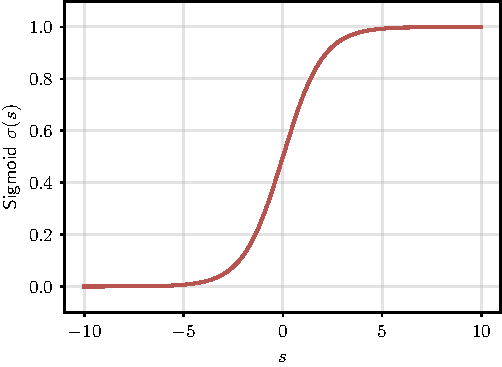
\includegraphics[width=0.6\textwidth]{images/sigmoid.pdf}
    \caption{Plot of the sigmoid function. Note that $\sigma(0)=0.5$.}
    \label{fig:sigmoid}
\end{SCfigure}

The \textbf{binary logistic regression} model is obtained by combining a one-dimensional linear model with a sigmoid rescaling of the output:
%
$$
f(\mathbf{x})=\sigma\left(\mathbf{w}^\top\mathbf{x}+b\right)
$$
%
The cross-entropy similarly simplifies to:

\vspace{1em}
\begin{equation}
\text{CE}(\hat{y},y) = \eqnmarkbox[drawred]{node}{-y\log(\hat{y})} \eqnmarkbox[drawblue]{node2}{-(1-y)\log(1-\hat{y})}
\end{equation}
\annotate[yshift=1em]{above,left}{node}{Loss for class $1$}
\annotate[yshift=1em]{above,right}{node2}{Loss for class $2$}

Hence, in the binary classification case we can solve the problem with two equivalent approaches: (a) a two-valued model with the standard softmax, or (b) a simplified one-valued output with a sigmoid output transformation. 

As an interesting side-note, consider the gradient of the binary logistic regression model with respect to $\mathbf{w}$ (a similar gradient can also be written for the standard multi-class case):
%
$$
\nabla \text{CE}(f(\mathbf{x}),y) = (f(\mathbf{x})-y)\mathbf{x}
$$
%
Note the similarity with the gradient of a standard linear model for regression. This similarity can be further understood by rewriting our model as:

\vspace{1em}
\begin{equation}
\eqnmarkbox[drawred]{node}{\mathbf{w}^\top \mathbf{x}+b}=\eqnmarkbox[drawblue]{node2}{\log\left(\frac{y}{1-y}\right)}
\end{equation}
\annotate[yshift=1em]{above,left}{node}{Logits}
\annotate[yshift=1em]{above,right}{node2}{Sigmoid inverse: $\sigma^{-1}(y)$}

This clarifies why we were referring to the model as a “linear model” for classification: we can always rewrite it as a purely linear model in terms of a non-linear transformation of the output (in this case, the inverse of the sigmoid, also known as the \textbf{log-odds}). In fact, the logistic regression model is part of a broader family of models extending this idea, called \textbf{generalized linear models}. For the curious reader, the name of the logit can be understood in this context in reference to the probit function.\footnote{\url{https://en.wikipedia.org/wiki/Probit}}

\subsection{The logsumexp trick} 

\addteacup This is a more technical subsection that clarifies an implementation aspect of what we described up to now. Looking at frameworks like TensorFlow or PyTorch, we can find multiple existing implementations of the cross-entropy loss, based on whether the output is described as an integer or as a one-hot encoded vector. This can be understood easily, as we have already seen that we can formulate the cross-entropy loss in both cases. However, we can also find variants that accept logits instead of the softmax-normalized outputs, as shown in Box \ref{code:cross_entropy}.

\begin{mypy}{Cross entropy losses in PyTorch. Some losses are only defined starting from the logits of the model, instead of the post-softmax output. These are the \textit{functional} variants of the losses - equivalent object-oriented variants are also present in most frameworks.}{code:cross_entropy}
# Binary cross-entropy
torch.nn.functional.binary_cross_entropy
# Binary cross-entropy accepting logits
torch.nn.functional.binary_cross_entropy_with_logits
# Standard cross-entropy, only works with logits
torch.nn.functional.cross_entropy
# Cross-entropy accepting log f(x) as inputs
torch.nn.functional.nll_loss
\end{mypy}

To understand why we would need this, consider the $i$-th term of the cross-entropy in terms of the logits $\mathbf{p}$:
%
$$
- \log\left( \frac{\exp{p_i}}{\sum_j \exp{p_j}} \right) \,.
$$
%
This term can give rise to several numerical issues, notably due to the interplay between the (potentially unbounded) logits and the exponentiation. To solve this, we first rewrite it as:
%
$$
- \log\left( \frac{\exp{p_i}}{\sum_j \exp{p_j}} \right) = -p_i + \underbrace{\log\left(\sum_j \exp p_j\right)}_{\triangleq \; \text{logsumexp}(\mathbf{p})}
$$
%
The first term does not suffer from instabilities, while the second term (the \textbf{logsumexp} of the logits) is a function of the entire logits’ vector, and it can be shown to be invariant for a given scalar $c \ge 0$ in the following sense:\footnote{\url{https://gregorygundersen.com/blog/2020/02/09/log-sum-exp/}}
%
$$
\text{logsumexp}(\mathbf{p})=\text{logsumexp}(\mathbf{p} - c) +c
$$
%
Note that $\nabla \text{softmax}(\bullet) = \text{logsumexp}(\bullet)$. By taking $c = \max(\mathbf{p})$ we can prevent numerical problems by bounding the maximum logit value at $0$. However, this is only possible if we have access to the original logits, which is why numerically stable variants of the cross-entropy require them as inputs. This creates a little amount of ambiguity, in that the softmax can now be included as either part of the model, or as part of the loss function.

\subsection{Calibration and classification}

We close the chapter by briefly discussing the important topic of \textbf{calibration} of the classifier. To understand it, consider the following fact: although our model provides an entire distribution over the possible classes, our training criterion only targets the maximization of the true class. Hence, the following sentence is justified:

\begin{quote}The predicted class of $f(\mathbf{x})$ is $\underset{i}{\arg\max} \; \idx{f(\mathbf{x})}{i}$.\end{quote}

Instead, this more general sentence might not be correct:

\begin{quote} The probability of $\mathbf{x}$ being of class $i$ is $\idx{f(\mathbf{x})}{i}$.\end{quote}

When the confidence scores of the network match the probability of a given prediction being correct, we say the network’s outputs are \textbf{calibrated}.

\begin{definition}[Calibration]
A classification model $f(\mathbf{x})$ giving in output the class probabilities is said to be calibrated if the following holds for any possible prediction:
%
$$
\idx{f(\mathbf{x})}{i} = p(y=i \;\vert\; \mathbf{x})
$$
%
\end{definition}

Although the cross entropy should recover the conditional probability distribution over an unrestricted class of models and in the limit of infinite data \cite{hastie2009elements}, in practice the mismatch between the two may be high \cite{blasiok2024does}, especially for the more complex models we will introduce later on.

To understand the difference between accuracy and calibration, consider these two scenarios. First, consider a binary classification model that has perfect accuracy, but always predicts the true class with $0.8$ confidence. In this case, the model is clearly \textit{underconfident} in its predictions, since by looking at the confidence we may assume that $20\%$ of them would be incorrect. Second, consider a $4$ class problem with perfectly balanced classes, with a model that always predict $[0.25, 025, 0.25, 0.25]$. In this case, the model is perfectly calibrated, but useless from the point of view of accuracy.

Having access to a calibrated model is very important in situations in which different predictions may have different costs. This can be formalized by defining a so-called \textit{cost matrix} assigning a cost $C_{ij}$ for any input of class $i$ predicted as class $j$. A standard example is a binary classification problem having the matrix of costs shown in Table \ref{tab:cost_matrix}.

%
\begin{table}[h]
\centering
\caption{Example of cost matrix for a classification problem having asymmetric costs of misclassification.}
\label{tab:cost_matrix}
\begin{tabular}{@{}lcc@{}}
\toprule
 & True class 0 & True class 1 \\ \midrule
Predicted class 0 & 0 & 10 \\
Predicted class 1 & 1 & 0 \\ \bottomrule
\end{tabular}
\end{table}

We can interpret Table \ref{tab:cost_matrix} as follows: making a correct prediction incurs no cost, while making a false negative mistake (0 instead of 1) is 10 times more costly than making a false positive mistake. As an example, an incorrect false negative mistake in a medical diagnosis is much worse than a false positive error, in which a further test may correct the mistake. A calibrated model can help us in better estimating the average risk of its deployment, and to fine-tune our balance of false positive and false negative mistakes.

To see this, denote by $\mathbf{C} \sim (m, m)$ the generic matrix of costs for a multiclass problem (like the $2\times2$ matrix in Table \ref{tab:cost_matrix}). The rational choice is to select a class which minimizes the expected cost based on the scores assigned by our model:
%
$$
\underset{i}{\arg\min} \sum_{j=1}^m C_{ij} \idx{f(\mathbf{x})}{j}
$$
%
If $C_{ij} = 1$ whenever $i \neq j$ and $0$ otherwise, this reduces to selecting the argmax of $f$, but for a general matrix of costs the choice of predicted class will be influenced by the relative costs of  making specific mistakes. This is a simple example of \textbf{decision theory} \cite{bishop2006pattern}.

\subsection{Estimating the calibration error}

To estimate whether a model is calibrated we can bin its predictions, and compare its calibration to the accuracy in each bin. To this end, suppose we split the interval $[0,1]$ into $b$ equispaced bins, each of size $1/b$. Take a validation set of size $n$, and denote by $\mathcal{B}_i$ the elements whose confidence falls into bin $i$. For each bin, we can further compute the average confidence $p_i$ of the model (which will be, approximately, in the middle of the bin), and the average accuracy $a_i$. Plotting the set of pairs $(a_i, p_i)$ on an histogram is called a \textbf{reliability diagram}, as shown in Figure \ref{fig:calibration_plot}. To have a single, scalar metric of calibration we can use, for example, the \textbf{expected calibration error} (ECE):

\begin{SCfigure}
    \centering
    \hspace{1em}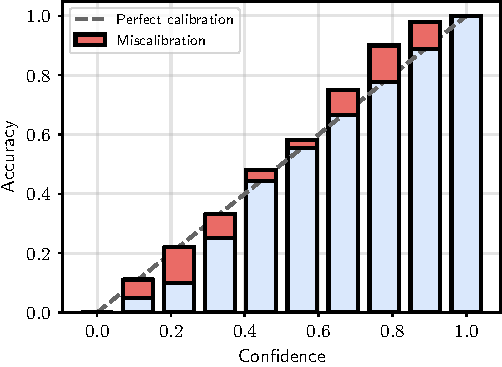
\includegraphics[width=0.5\textwidth]{images/reliability_plot.pdf}
    \caption{An example of reliability plot with $b=10$ bins. The blue bars show the average accuracy of the model on that bin, while the red bars show the miscalibration for the bin, which can be either under-confident (below the diagonal) or over-confident (above the diagonal). The weighted sum of the red blocks is the ECE in \eqref{eq:ece}.}
    \label{fig:calibration_plot}
\end{SCfigure}

\begin{equation}
\displaystyle\text{ECE}= \sum_i \eqnmarkbox[drawred]{node2}{\frac{\lvert\mathcal{B}_i\rvert}{n}} \eqnmarkbox[drawblue]{node}{\left|a_i - p_i\right|}
\label{eq:ece}
\end{equation}
\annotate[yshift=1em]{above,right}{node}{Calibration for bin $i$}
\annotate[yshift=-1em]{below,right}{node2}{Fraction of validation set falling into bin $i$}

\vspace{1em}
Other metrics, such as the maximum over the bins, are also possible. If the model is found to be uncalibrated, modifications need to be made. Examples include rescaling the predictions via temperature scaling \cite{guo2017calibration} or optimizing with a different loss function such as the focal loss \cite{mukhoti2020calibrating}.

We close by mentioning an alternative to direct calibration of the model, called \textbf{conformal prediction}, which has become popular recently \cite{angelopoulos2021gentle}. Suppose we fix a threshold $\gamma$, and we take the set of classes predicted by the model whose corresponding probability is higher than $\gamma$:
%
\begin{equation}
\mathcal{C}(\mathbf{x}) = \left\{ i \mid \idx{f(\mathbf{x})}{i} > \gamma \right\}
\label{eq:support_set}
\end{equation}

\begin{SCfigure}
    \centering
    \hspace{1em}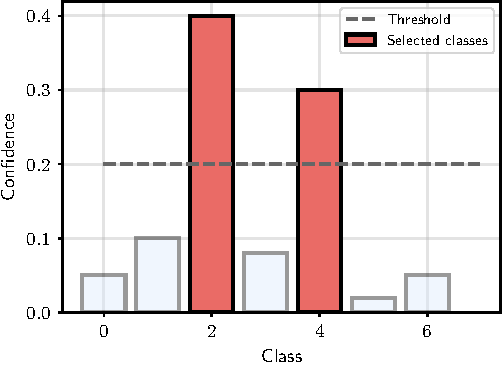
\includegraphics[width=0.5\textwidth]{images/conformal_prediction.pdf}
    \caption{Calibration by turning the model's output into a set: we return all classes whose predicted probability exceeds a given threshold. By properly selecting the threshold we can bound the probability of the true class being found in the output set.}
    \label{fig:conformal_prediction}
\end{SCfigure}

i.e., the answer of the model is now a \textit{set} $\mathcal{C}(\mathbf{x})$ of potential classes. An example is shown in Figure \ref{fig:conformal_prediction}. The idea of conformal prediction is to select the minimum $\gamma$ such that the probability of finding the correct class $y$ in the set is higher than a user-defined error $\alpha$:\footnote{Note that it is always possible to satisfy this property by selecting $\gamma = 0$, i.e., including all classes in the output set.}
%
\begin{equation}
p(y \in \mathcal{C}(\mathbf{x})) \ge 1 -\alpha
\label{eq:conformal_prediction}
\end{equation}
%
Intuitively, there is an inversely proportional relation between $\gamma$ and $\alpha$. Conformal prediction provides automatic algorithms to guarantee \eqref{eq:conformal_prediction} at the cost of not having a single class in output anymore.

\section*{From theory to practice}

\begin{wrapfigure}{r}{3.0cm}
\vspace{-3em}
\includegraphics[width=3.0cm]{images/shutterstock_2075221579.jpg}
\vspace{-6em}
\end{wrapfigure}

From Chapter \ref{chap:preliminaries} you should have a good grasp of NumPy, JAX, and PyTorch's \mintinline{python}{torch.tensor}. They are all okay for this chapter, and nothing else is required.

I suggest a short exercise to let you train your first differentiable model:

\begin{enumerate}
\item Load a toy dataset: for example, one of those contained in scikit-learn datasets module.\footnote{\url{https://scikit-elearn.org/stable/datasets/toy_dataset.html}}
\item Build a linear model (for regression or classification depending on the dataset). Think about how to make the code as modular as possible: as we will see, you will need at least two functions, one for initializing the parameters of the model and one for computing the model's predictions.
\end{enumerate}

\begin{enumerate}\addtocounter{enumi}{2}
\item Train the model via gradient descent. For now you can compute the gradients manually: try to imagine how you can make also this part modular, i.e., how do you change the gradient's computation if you want to dynamically add or remove the bias from a model?
\item Plot the loss function and the accuracy on an independent test set. If you know some standard machine learning, you can compare the results to other supervised learning models, such as a decision tree or a $k$-NN, always using scikit-learn.
\end{enumerate}